\begin{figure}[t!] 
        \centering
        \begin{subfigure}[b]{1.8in}
                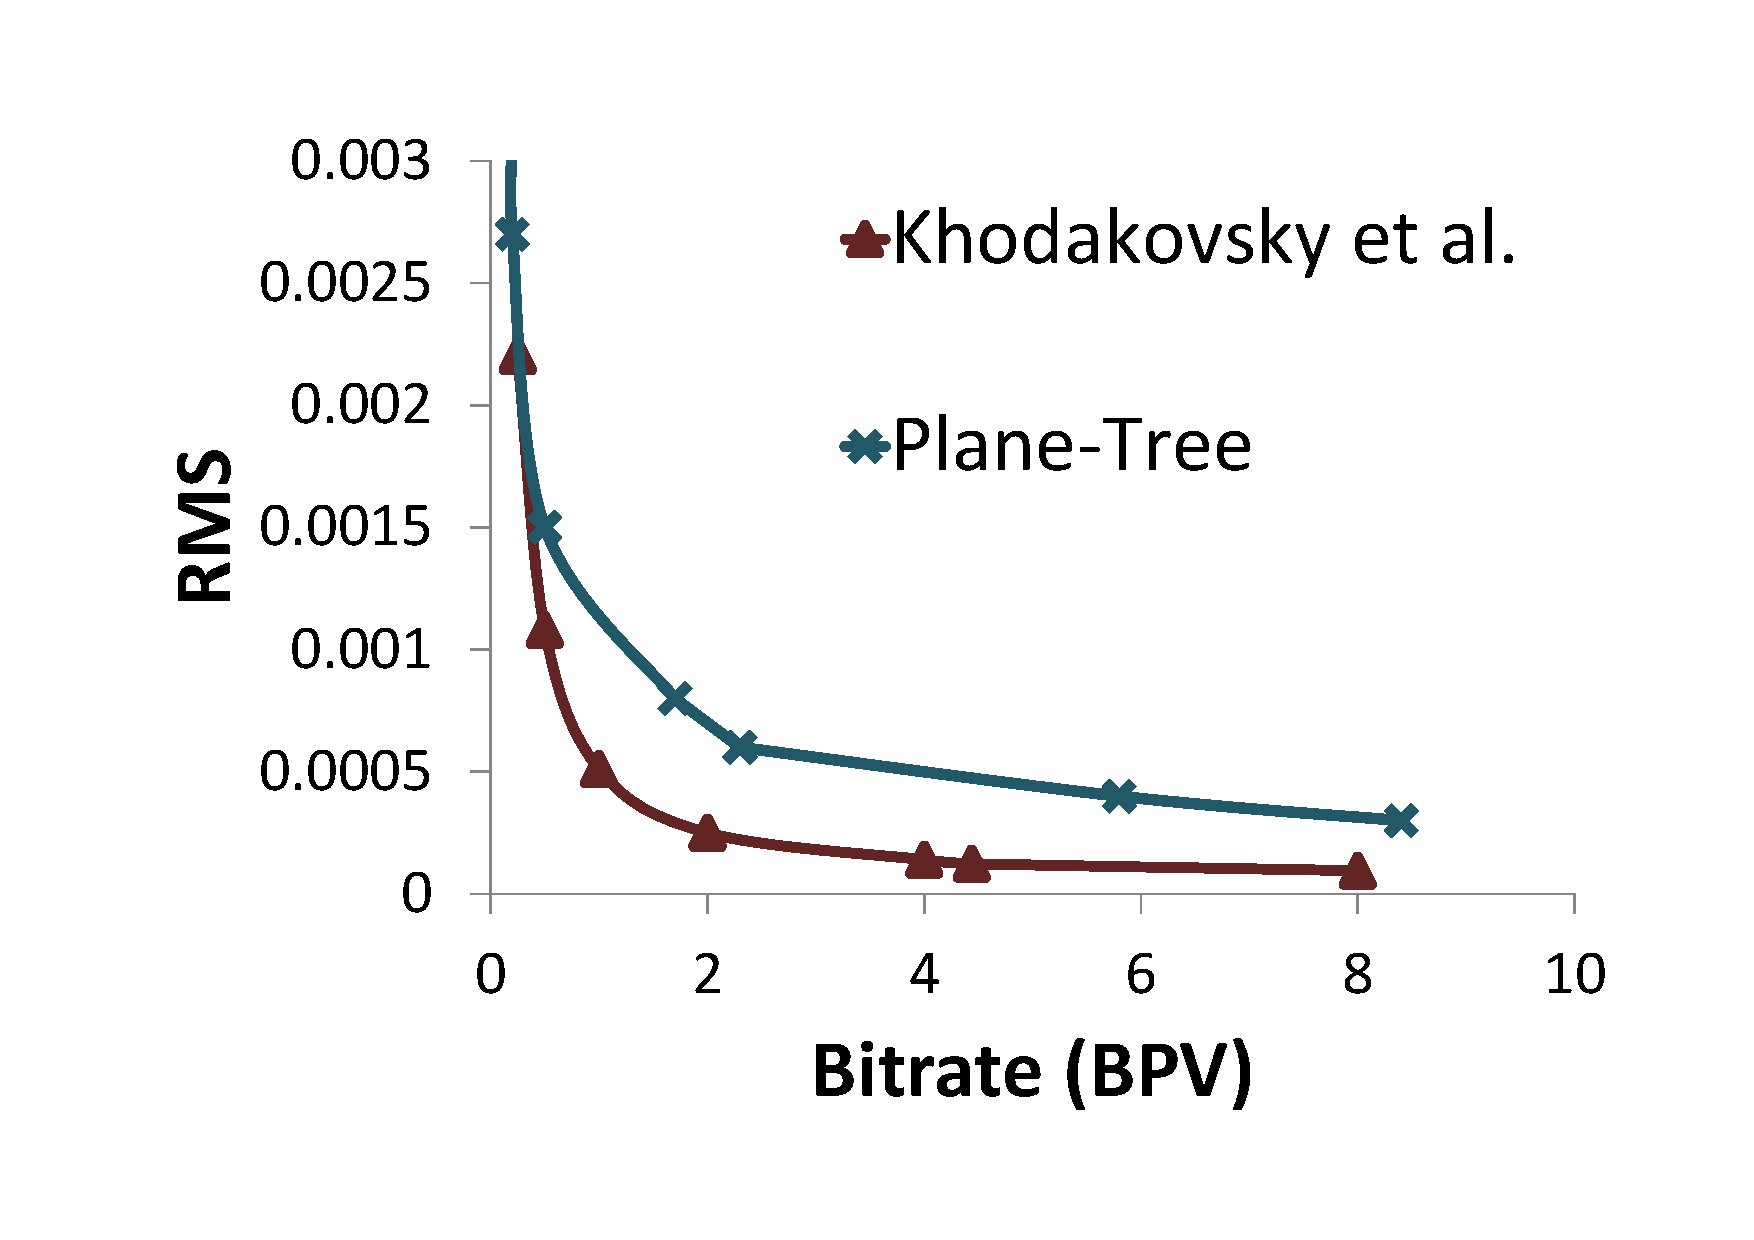
\includegraphics[width=1.8in]{images/results/compression/bunnysota}
                \caption{Bunny Model}
                \label{fig:SA_BUNNY}
        \end{subfigure}%
        \begin{subfigure}[b]{1.8in}
                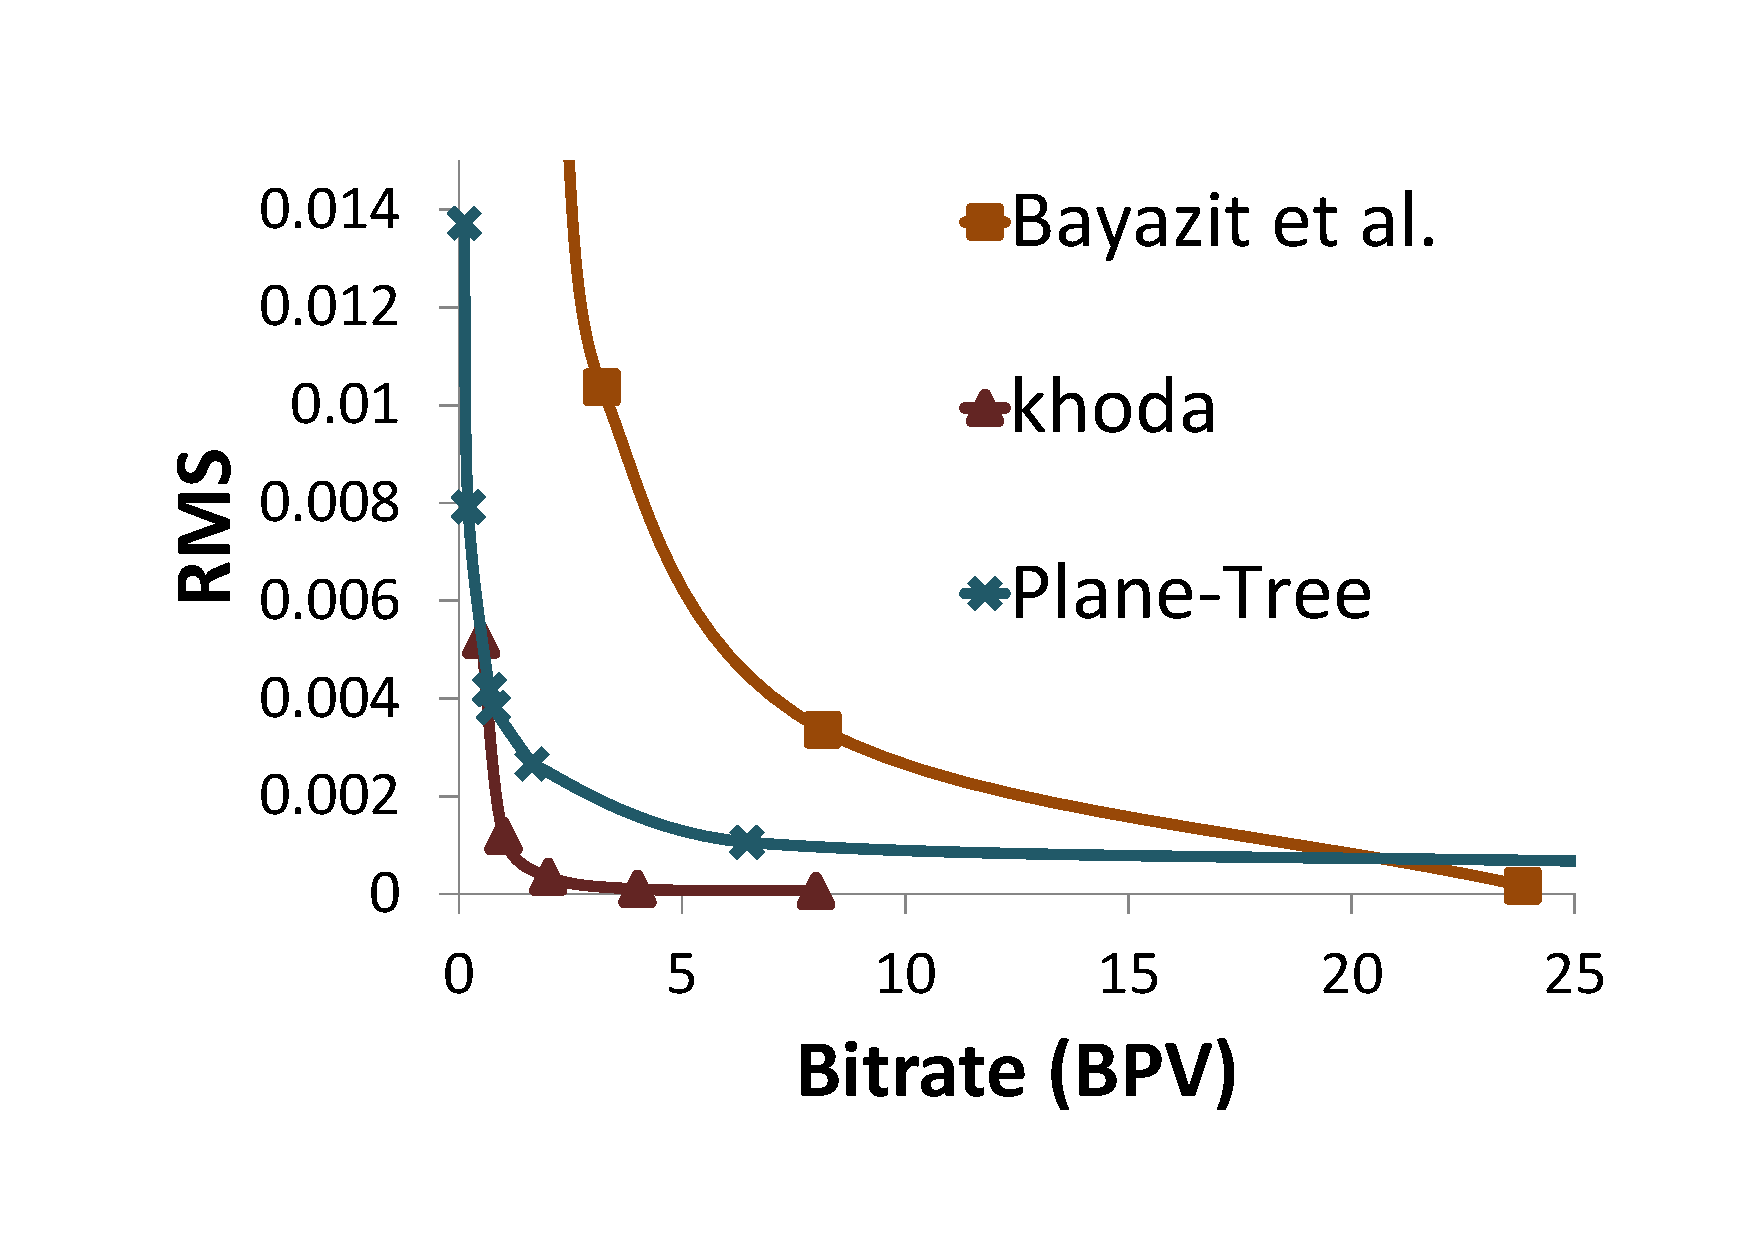
\includegraphics[width=1.8in]{images/results/compression/fandisksota}
                \caption{Fandisk Model}
                \label{fig:SA_FANDISK}
        \end{subfigure}
        
        \begin{subfigure}[b]{1.8in}
                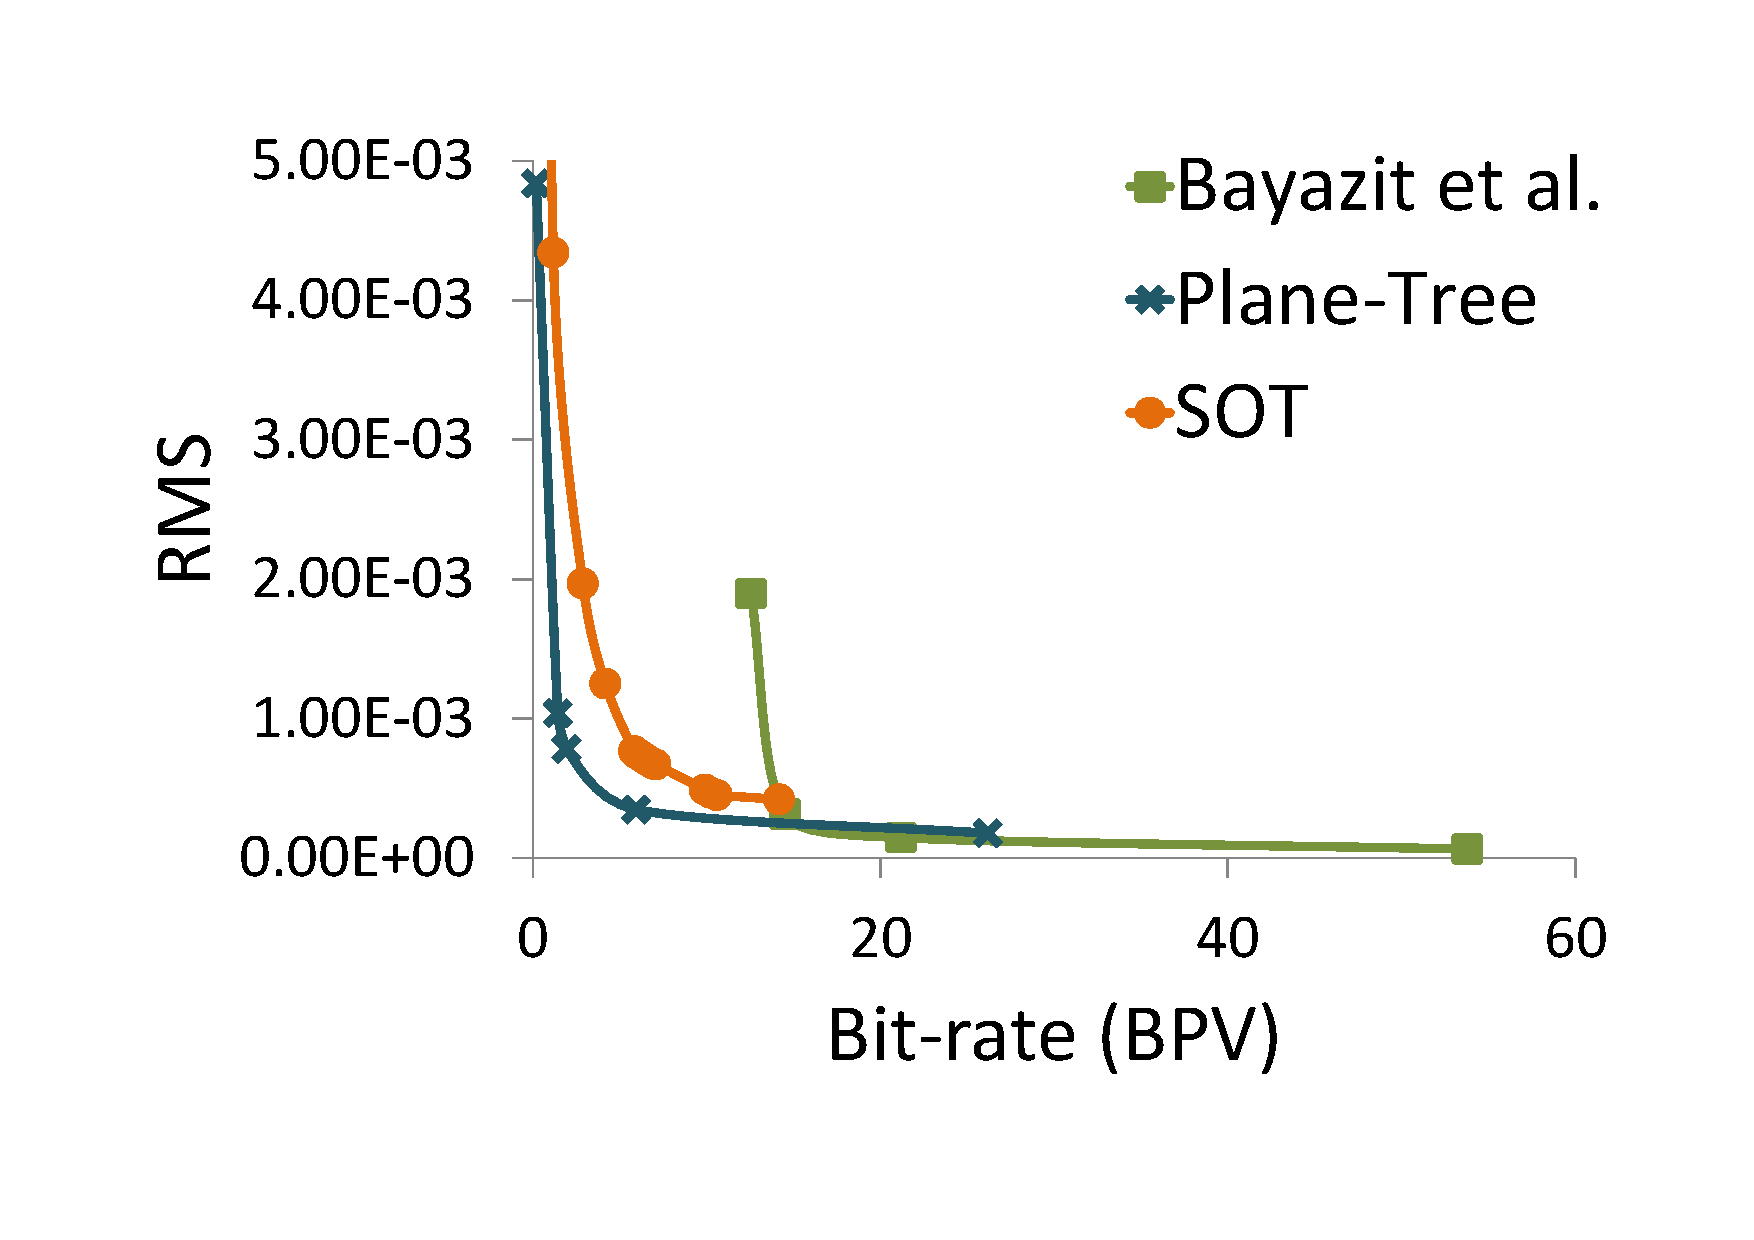
\includegraphics[width=1.8in]{images/results/compression/horsesota}
                \caption{Horse Model}
                \label{fig:SA_HORSE}
        \end{subfigure}%
        \begin{subfigure}[b]{1.8in}
                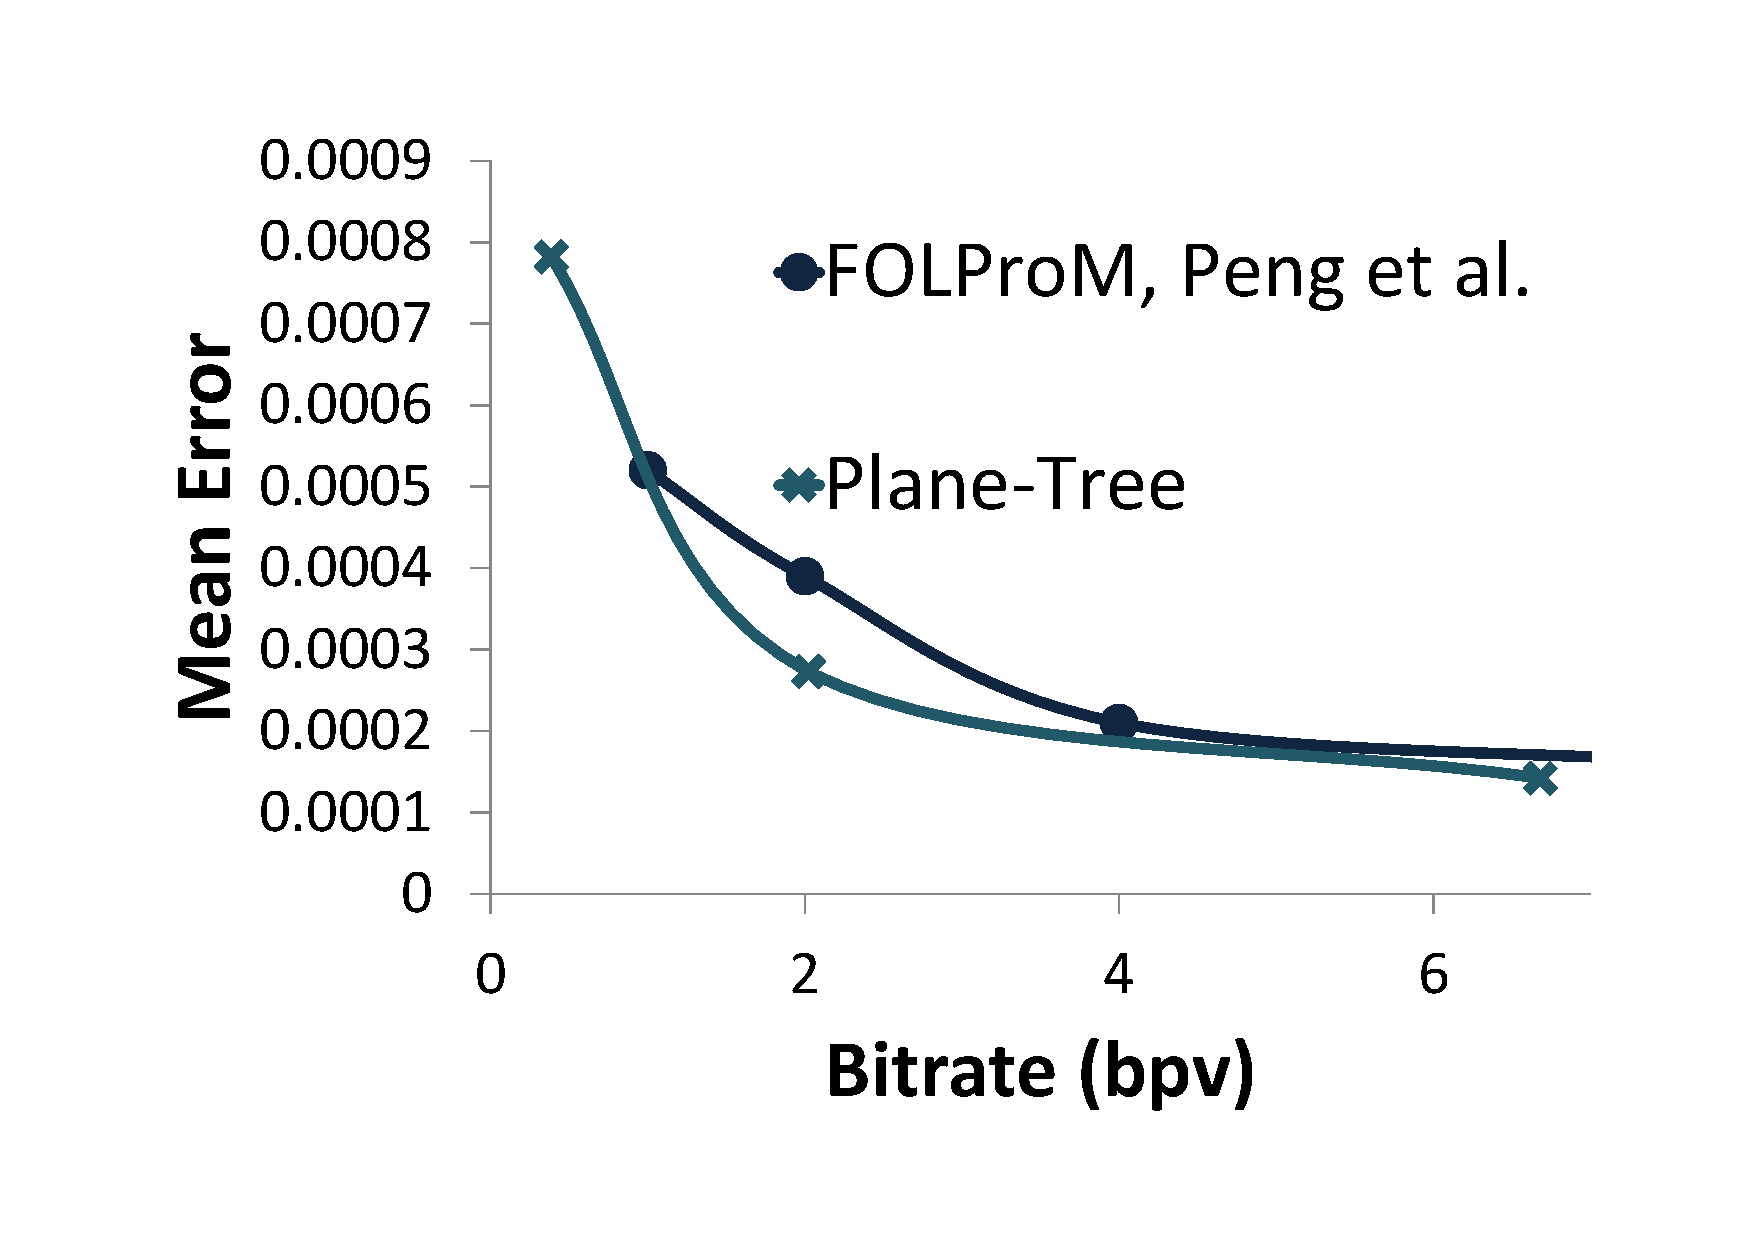
\includegraphics[width=1.8in]{images/results/compression/rabbitsota}
                \caption{Rabbit Model}
                \label{fig:SA_RABBIT}
        \end{subfigure}
       \caption{Rate-Distortion graphs comparing the Plane-Tree to different state of the art codecs.}
       \label{fig:SOTAEXPS}
\end{figure}

In figures \ref{fig:SA_BUNNY}, \ref{fig:SA_FANDISK} and \ref{fig:SA_HORSE} we compare the Plane-Tree with the state of the art transform methods by Bayazit et al \cite{Bayazit103DMesh} and Khodakovsky et al \cite{Khodakovsky00Progressive}. Figure \ref{fig:SA_BUNNY} shows the Plane-Tree has similar distortion compared with the method by Khodakovsky at low-bitrates, whilst being competitive with it up to much higher bitrates. \\

Figure \ref{fig:SA_FANDISK} shows similar results compared with Khodakovsky's method, it also shows the Plane-Tree outperforms the spectral compression method by Bayazit et al at both low and mid level bitrates. Figure \ref{fig:SA_HORSE} shows how the much simpler Plane-Tree method outperforms the transform based method of Bayazit et al. Whilst our method remains competitive at higher bitrates, it outperforms the method by Bayazit at lower bitrates. \\

Finally the Plane-Tree is compared with the state of the art low-bitrate compression system FOLProM \cite{Peng10Feature} using the mean error metric. It can be seen that at low-bitrates (below 2 bits per vertex), the Plane-Tree method outperforms this state of the art low-bitrate compression system. \\